\documentclass{article}
\usepackage{fancyhdr}
\usepackage{datetime}
\usepackage{parskip}
\usepackage{graphicx}

\newdateformat{monthyeardate}{\monthname[\THEMONTH], \THEYEAR}

\pagestyle{fancy}

\fancyhf{}
\fancyfoot[L]{University of Oulu. \monthyeardate\today}

\lhead{IoT Data Analytics}
\rhead{Page \thepage}

\title{
Exercise 2: IoT Data Analytics
\bigskip
\author{Andrei Golubev 2621924 \\ Hassan Shaheen 2600602}
\date{\parbox{\linewidth}{\centering
  \endgraf\bigskip
  University of Oulu, Oulu, Finland
  \endgraf\monthyeardate\today}}
}

\setlength{\parindent}{0pt}

\begin{document}
\maketitle
\thispagestyle{empty}
\newpage

\section{Visualization}

Visualization implementation can be divided into two separate tasks: data preparation and actual
implementation. The first one is required when the data is not ready for the use (e.g. collected
from different sources or in a wrong format), which is usually the case in real world data
visualization. The second relies on the use case and research topic and should ideally simplify data
analysis. In the following subsections we describe briefly the visualization approach details.

\subsection{Data preparation}

There are two primary data files that need to be considered: sensor measurements (temperature, pir,
co2, etc.) and sensor GPS coordinates.

We perform the following preprocessing on the \textbf{Sensor GPS coordinates} file:

* Move out all unnecessary information (e.g. Tellus area GPS coordinates).

* Convert XLSX format file into plain CSV.

* Unify device id format between this file and sensor measurements file.

* Convert GPS coordinates into relative to Tellus area coordinates (this is a necessary step for
futher visualization and explained below).

\textbf{Sensor measurements} file is also preprocessed:

* Only required information is left: device ids (required for later localization), timestamps, pir
readings.

* The whole data file is split into \textit{monthly} data (a single CSV contains 1 month of sensor
measurements). In our use case, monthly separation is sufficient and the benefits of such a split
are not to be ignored as we gain reduced the memory footprint during visualization and as well as
significant speed up during parsing.

With the described actions in mind, we are able to successfully implement visualization that gives
us a good base for future analysis.

\subsection{Visualization implementation}

We visualize the sensor measurements (PIR data) by drawing it on a 2D image. This is done via a
mapping from GPS coordinates of sensors that are converted into relative to Tellus area and then
converted into image coordinates relative to used Tellus map found at [1]. Figures 1 and 2 show the
map and the corresponding area annotation.

We draw sensor layer on top of the image-based map, with sensors by default being represented by
pixel dots (see Figure 3.).

To visualize PIR measurements we use simple transparent circles where the radius of the circle is
proportional to the PIR number. To represent measurements over time, we bundle individual 2D Tellus
map images (with sensor data layer) into a GIF. We use \textit{1 hour} time precision so any two
consecutive maps (images) in the GIF differ by one hour and thus the PIR data for the whole hour is
aggregated into a single image. Figure 4 shows snapshots from the GIF for some random time period.

\begin{figure}[ht!]
  \centering
  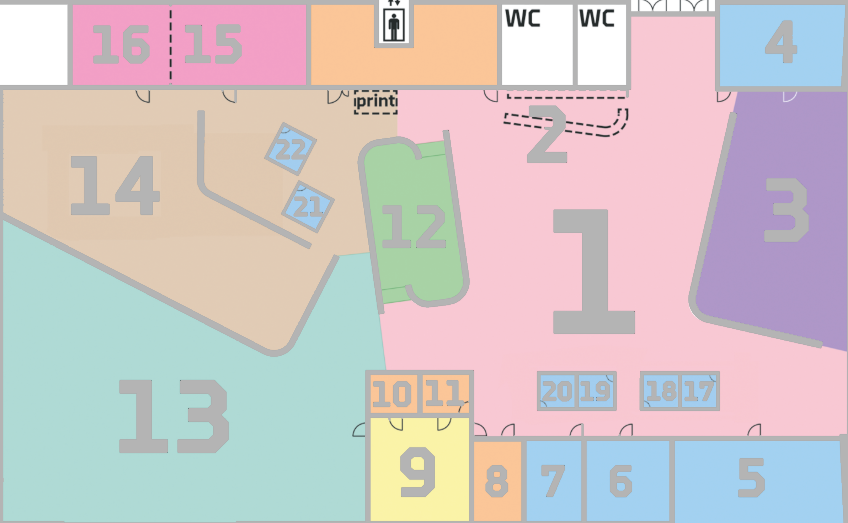
\includegraphics[width=90mm]{./tellus_map.png}
  \caption{Tellus map. Modified [1]}
\end{figure}

\begin{figure}[ht!]
  \centering
  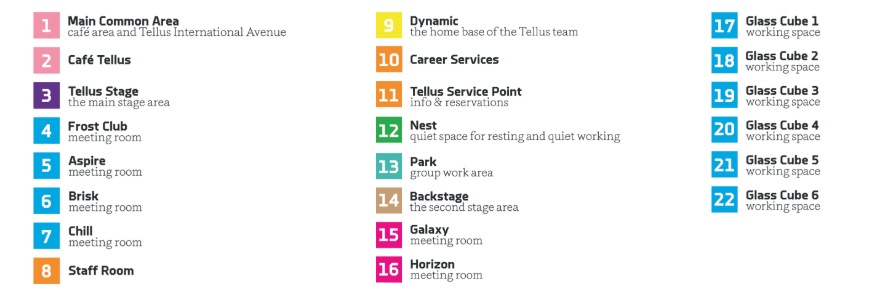
\includegraphics[width=90mm]{./tellus_map_annotation.png}
  \caption{Tellus map annotation [1]}
\end{figure}

\begin{figure}[ht!]
  \centering
  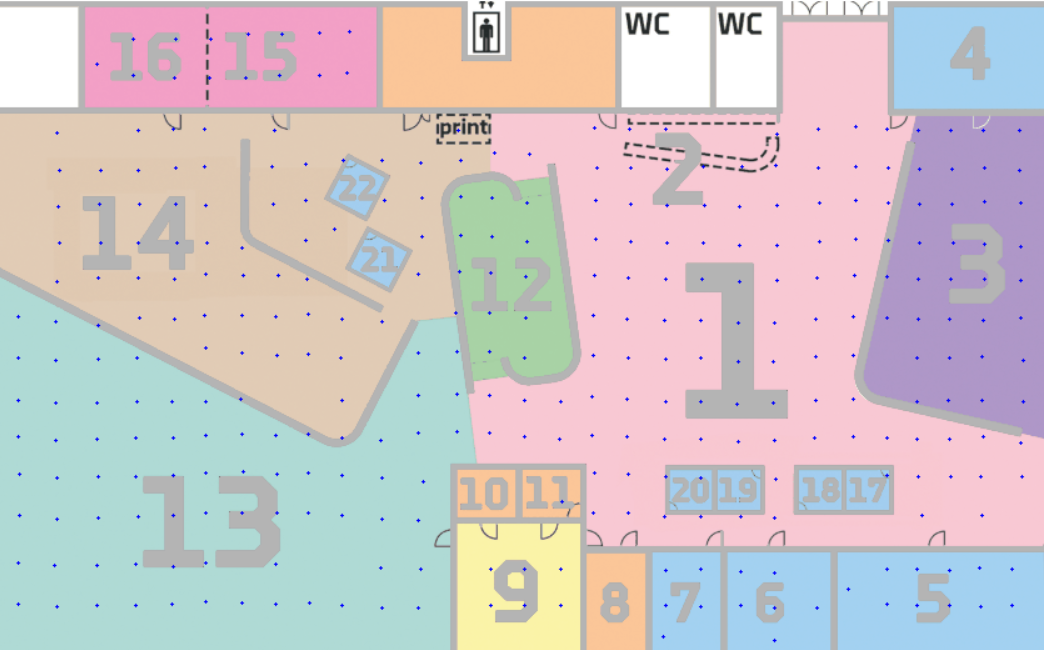
\includegraphics[width=90mm]{./tellus_map_sensor_locations.png}
  \caption{Tellus map with sensor locations}
\end{figure}

\begin{figure}[ht!]
  \centering
  \begin{minipage}{.5\textwidth}
    \centering
    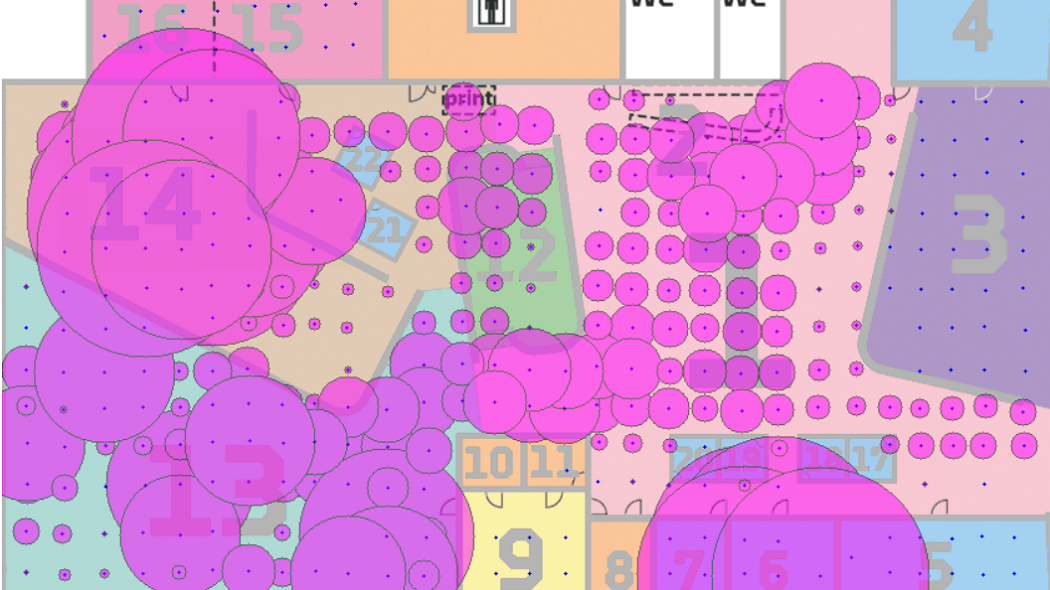
\includegraphics[width=.95\linewidth]{./tellus_map_sensor_data_1.png}
  \end{minipage}%
  \begin{minipage}{.5\textwidth}
    \centering
    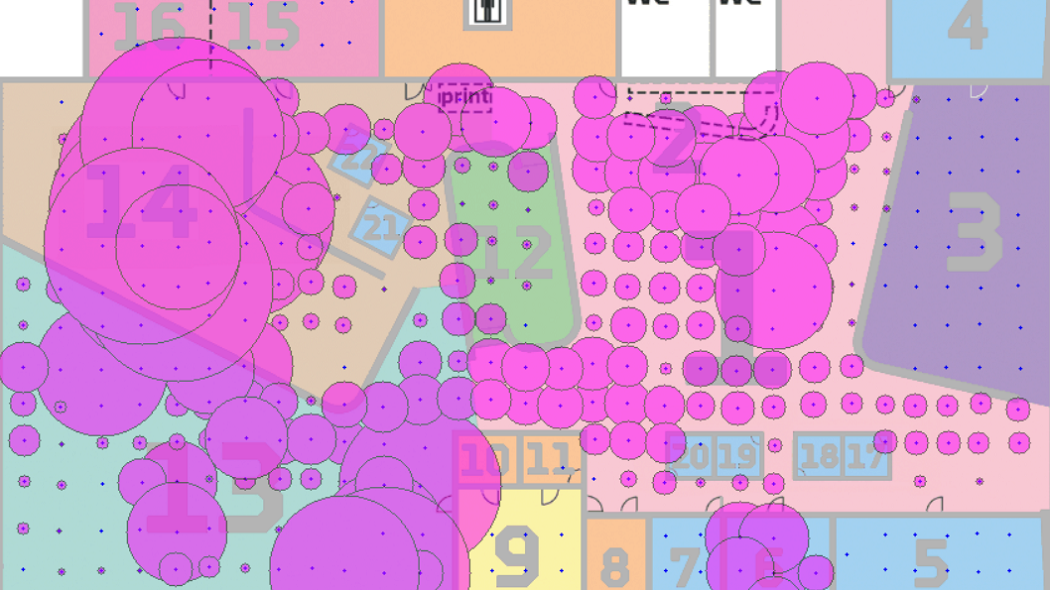
\includegraphics[width=.95\linewidth]{./tellus_map_sensor_data_2.png}
  \end{minipage}
  \caption{Tellus map snapshots with sensor measurements layer added}
\end{figure}

\section{Seasonal variations}

To investigate the seasonal variations, we are analysing the difference of movement data among
random weeks, exam weeks, and holiday weeks.

\subsection{Week variations}

In our analysis, we found out that there is a clear pattern in movement data during a single day.
During weekdays movement start around 8 am and from 10 am to 4 pm Tellus is at its full capacity.
After 4 pm it starts decreasing and after 8 pm there is very little movement, the pattern is the
same until Friday. But the weekends are different, on Saturday’s movement starts after 10 pm and it
visible up to 7 pm however the average movement is quite low as compared to weekdays. As the
university is closed on Sundays there is very little movement. There are exceptions on Sundays we
found out that on some specific Sundays due to some event or meeting in Tellus stage (Area 3) or
meeting rooms the numbers can vary but the overall pattern is the same. From the visualization, we
can see that area 1 (Main common area) and area 13 (Group work area) are mostly occupied.

\subsection{Exam weeks}

By comparing random weeks with exam weeks, we identified that there is no clear difference in the
pattern on  weekdays and weekends, they are almost identical in both weeks.

\subsection{Holiday weeks}

During Christmas time (in 2017), there is also a very understandable pattern: until 23rd of December
there are still many people in Tellus; from 23rd to 25th the Tellus is almost completely empty; on
26th of December Tellus Stage is occupied by approximately 50 people (we believe it might be a small
Christmas party); from 27th Tellus slowly becomes occupied by a moderate amount of people.

During summer time the situation is the following:

- in June Tellus is still used but the amount of people is smaller than during a normal study week.

- in July Tellus is completely empty (with small amount of people ~10 at the beginning of the month
on 1st-4th of July).

- in August, the amount of people increases from zero and by the end of the month the whole Tellus
is used.

The situation is also rather deterministic: June being the month when students finish their study
period, July is the vacation month with almost no one around the campus (and students usually do
summer internships outside of the university), in August people start to return back from holidays
to engage into the university life.

\section{Future implications}

With the help of movement data, we can analyze in the future which area is occupied the most and
require expansion. As described above, we discovered in our analysis that the most used areas are
Group work area and Main common area and the least used areas are meeting rooms. This will help us
during the re-design of current Tellus space or when designing a new one.

\subsection{Suggested improvements}

We believe that the main improvements should focus on allocating more space in commonly used
areas such as Group work area and Main common area. Meeting rooms seem to be empty most of the time
which is not very space efficient, a better approach to space manipulation should be used, for
example, having a meeting room space as part of a bigger area by default, with the ability to
separate the room whenever needed: this can be achieved with the help of \textit{transparent sliding
doors} instead of traditional stationary walls.

Analysing holiday times, we clearly see that the Tellus area is rather unused. Maybe it makes sense
to transform Tellus area from business/study oriented into something leisure-like by e.g. installing
a temporary cinema equipment or booths with games (table, sport, computer games), etc. We think that
it may be interesting for people who remain in Oulu during Christmas time or wish to spend time in
Tellus during summer holidays.

\subsection{Movement data application}

One potential application of movement data could be real-time Tellus map that shows the sitting
capacity of Tellus, right now one of the biggest challenges is that we need to manually check for
available space. If there can be a screen outside Tellus showing the current stats of its capacity.
If certain booths are empty? Is there space available in the group work area? This will be very
beneficial, it will reduce the traffic in Tellus and save users the manual check.


\section{References}

1. Tellus map. URL: https://www.oulu.fi/tellusarena/description-map

\end{document}
